\documentclass[12pt,a4paper,openright,twoside]{book}
\usepackage[italian]{babel}
\usepackage[utf8]{inputenc}
\usepackage{fancyhdr}
\usepackage{indentfirst}
\usepackage{graphicx}
\usepackage{verbatim}

\pagestyle{fancy}


\oddsidemargin=30pt
\evensidemargin=20pt


% Sillabazione
\hyphenation{}

% Intestazione e piè di pagina
\pagestyle{fancy}\addtolength{\headwidth}{20pt}
\renewcommand{\chaptermark}[1]{\markboth{\thechapter.\ #1}{}}
\renewcommand{\sectionmark}[1]{\markright{\thesection \ #1}{}}
\rhead[\fancyplain{}{\bfseries\leftmark}]{\fancyplain{}{\bfseries\thepage}}
\cfoot{}

% Interlinea
\linespread{1.6}

\begin{document}

%
% Dedica
%
\begin{titlepage}
  % No numero di pagina
  \thispagestyle{empty}
  \topmargin=6.5cm
  \raggedleft
  \large \em A Chiara
  \newpage
  % Non numera l'ultima pagina a sinistra.
  \clearpage{\pagestyle{empty}\cleardoublepage}
\end{titlepage}


\pagenumbering{roman}

\chapter*{Introduzione}
\rhead[\fancyplain{}{\bfseries
INTRODUZIONE}]{\fancyplain{}{\bfseries\thepage}}
\lhead[\fancyplain{}{\bfseries\thepage}]{\fancyplain{}{\bfseries
INTRODUZIONE}}
\addcontentsline{toc}{chapter}{Introduzione}

TODO

% Non numera l'ultima pagina a sinistra.
\clearpage{\pagestyle{empty}\cleardoublepage}

% Indice
\tableofcontents
\rhead[\fancyplain{}{\bfseries\leftmark}]{\fancyplain{}{\bfseries\thepage}}
\lhead[\fancyplain{}{\bfseries\thepage}]{\fancyplain{}{\bfseries
INDICE}}
% Non numera l'ultima pagina a sinistra.
\clearpage{\pagestyle{empty}\cleardoublepage}

\chapter{Definizione del problema}
\pagenumbering{arabic} Def problema: in un ambiente con numerose reti
senza fili eterogenee per tecnologia, politica di accesso e proprietà,
si vuole dare a un dispositivo di rete mobile la possibilità di
attraversare i campi d'azione delle suddette reti utilizzando quella
che in ogni momento risulti offrire l'accesso migliore ai
servizi. Tale dispositivo mobile viene chiamato Mobile Node (MN) e si
suppone sia dotato di più d'una interfaccia di rete senza fili. Dette
interfacce di rete (NIC) si potranno associare ognuna a una rete
differente e dovranno essere monitorate con continuità per determinare
in ogni momento quale di queste sia la più adatta ad effettuare
l'invio dei dati. La scelta di questa interfaccia designata si potrà
basare su numerosi criteri tra cui qualità del segnale radio,
percentuale di pacchetti persi, larghezza di banda offerta dal canale,
latenza di comunicazione, esigenze di sicurezza, eventuale costi
economici legati all'accesso alla rete e possibili preferenze
specificate direttamente dall'utente. L'insieme dei criteri di scelta
definisce le politiche di qualità del servizio (QoS) in uso, ovvero
l'insieme di regole e vincoli che devono essere rispettati per
garantire all'utente del MN un'esperienza soddisfacente di utilizzo
dei servizi. Le soluzioni dovranno fornire sia i meccanismi per
permettere all'utente, o alle applicazioni da lui utilizzate, di
specificare quali siano dette politiche, sia meccanismi che le
implementino.

TODO: immagine che mostri un MN che attraversa più reti e che mostra i
punti di handover.

\section{Punti critici}
\label{sec:punti-critici}
Le sezioni successive presentano gli aspetti critici del problema. La
bontà di una soluzione deve essere valutata sulla base di come risolve
le problematiche seguenti.

\subsection{Adattabilità}
Ogni applicazione in uso sul MN può avere le proprie esigenze di QoS,
che possono variare dalla necessità di utilizzare consistenti
quantitativi di banda alla necessità di avere una buona interattività,
misurata in termini di latenza di trasmissione dei dati. Un esempio
della prima classe di applicazioni possono essere i servizi di
Video-on-Demand (VoD), che offrono contenuti multimediali in
streaming, mentre un esempio della seconda classe è rappresentato dai
servizi Voice-over-IP (VoIP), che offrono la possibilità agli utenti
di comunicare tra di loro con chiamate audio/video sia individuali che
di gruppo. Ulteriori requisiti possono imporre un limite superiore
alla percentuale di pacchetti persi, per evitare che la qualità del
servizio non degradi oltre il limite dell'accettabile.

Le soluzioni dovranno quindi adattarsi alle necessità delle varie
applicazioni, cercando di rispettare le diverse politiche richieste da
ognuna.

\subsection{Monitoraggio}
Il concetto di qualità di servizio deve essere concretizzato in
un'insieme di limiti riguardanti metriche di comunicazione. Ad esempio
un'applicazione potrebbe richiedere che la comunicazione subisca una
perdita di pacchetti non superiore al 3\%; in questo caso
l'applicazione misura la qualità del servizio in termini di
percentuale di pacchetti persi, e impone su questa metrica un vincolo
del 3\%. Le soluzioni dovranno essere in grado di monitorare le
comunicazioni sulle varie interfacce dei MN per controllare che i
vincoli sulle metriche non vengano violati; questo richiede la
capacità di collezionare dati riguardanti queste varie metriche e la
capacità di prendere decisioni in base alle misurazioni effettuate e
alle politiche ricevute dall'applicazione. Nell'esempio precedente,
una soluzione che rilevi una percentuale di pacchetti persi superiore
al 3\% potrebbe decidere di utilizzare contemporaneamente due
interfacce di rete per limitare gli errori di trasmissione, posto che
le politiche specificate lo permettano.

\subsection{Handover}
\label{sec:handover}
Con \emph{handover} si intende il passaggio di associazione del Mobile
Node da una rete a un'altra. Lo scenario in cui le soluzioni si
troveranno ad operare sarà caratterizzato da un grado di libertà dei
MN molto ampio. Un possibile scenario è illustrato in \cite{bib:abc}:
un utente di MN comincia la comunicazione sulla rete domestica; dopo
un certo tempo esce di casa a comunicazione in corso, portando il MN
con sè. Durante il tragitto da casa alla fermata della metropolitana
il MN si disconnette dalla rete domestica e si associa alla rete
comunale, effettuando un primo handover. Quando pochi minuti più tardi
l'utente entra in metropolitana, il MN effettua un ulteriore handover
passando dalla rete comunale a quella della società dei trasporti
pubblici. Le soluzioni dovranno gestire handover di questo tipo in
maniera trasparente all'utente, ovvero senza che sia necessaria una
riconfigurazione manuale dell'applicazione o del dispositivo mobile, e
senza che venga intaccata la qualità del servizio.

L'handover è per sua natura un'operazione distruttiva che interrompe
le comunicazioni esistenti e richiede un tempo di completamento che
può arrivare all'ordine dei secondi. Tipicamente i passi che una NIC
deve completare per effettuare un handover sono:
\begin{enumerate}
\item scansione del canale per rilevare un nuovo access point,
\item associazione con il nuovo access point,
\item acquisizione di un nuovo indirizzo IP,
\item comunicazione del nuovo indirizzo IP ai vari corrispondenti, in
  modo che le comunicazioni possano continuare.
\end{enumerate}
I punti uno e due sono operazioni che appartengono al secondo livello
dello stack ISO/OSI, ovvero il livello \emph{data link}, e sono state
misurate sperimentalmente nell'ordine dei 50--400 ms
\cite{bib:misura-handoff-l2}. I punti tre e quattro sono operazioni
che appartengono al terzo livello dello stack ISO/OS, ovvero il
livello \emph{network}, e possono richiedere indicativamente almeno
300 ms \cite{bib:misura-handoff-dhcp}, perché l'assegnamento
dell'indirizzo IP da parte di un server DHCP e la comunicazione del
nuovo indirizzo a tutti gli host in contatto con il MN sono operazioni
legate alla latenza della rete.

Le soluzioni dovranno implementare meccanismi sia per ridurre questi
tempi in cui la connessione è inutilizzabile, sia per comunicare la
nuova identità del MN agli altri nodi. È importante notare che gli
altri nodi possono essere connessi a reti diverse da quella del MN e
quindi non sono applicabili meccanismi come broadcasting e
multicasting.

\subsection{Sicurezza}
In molti scenari domestici e aziendali la sicurezza della
comunicazione è spesso affidata alla sicurezza del medium in uso, ad
esempio il cavo ethernet o la crittografia della rete WiFi, e il
riconoscimento dell'identità dell'host è basata sull'indirizzo IP
dell'interfaccia di rete attiva. Queste assunzioni non sono più valide
nello scenario del problema in esame, dove numerosi MN con interfacce
di rete multiple eseguono numerosi handover attraverso reti senza
fili. Poiché queste reti verranno utilizzate da un grande numero di
individui che non possono avere relazioni di mutua fiducia, la
sicurezza è un problema centrale. Le soluzioni dovranno quindi fornire
sia meccanismi per garantire la riservatezza e l'integrità dei singoli
flussi di dati per ogni MN, sia meccanismi di identificazione e
autenticazione di ogni MN che sia indipendente dall'indirizzo IP della
rete di accesso.

\subsection{Praticità}
Nello scenario del problema sono coinvolte un gran numero di
tecnologie hardware e software che devono essere modificate il meno
possibile per permettere una realizzazione effettiva delle soluzioni
proposte in tempi e costi il più possibile contenuti.

In particolare è importante che le soluzioni siano in grado di
funzionare sui dispositivi hardware di rete esistenti, come interfacce
di rete, access point e router. Inoltre è vitale che la soluzione si
adatti ai più diversi scenari di topologia di rete, soprattutto in
quelle situazioni in cui esistono firewall e NAT che possono limitare
il traffico e la raggiungibilità degli host. Infine le applicazioni
software esistenti, dovrebbero essere in grado di funzionare senza
modifiche.

Per aiutare il passaggio graduale dell'utenza dalle soluzioni
tradizionali alle soluzioni proposte, è auspicabile che queste ultime
siano in grado di convivere con le prime utilizzando meccanismi di
fallback che garantiscano l'interoperabilità.

% Non numera l'ultima pagina a sinistra.
\clearpage{\pagestyle{empty}\cleardoublepage}

\chapter{Panoramica delle soluzioni}
\lhead[\fancyplain{}{\bfseries\thepage}]{\fancyplain{}{\bfseries\rightmark}}
L'obiettivo è di permettere a un MN di muoversi attraverso reti
wireless di natura eterogenea in maniera trasparente, ovvero senza
interrompere eventuali connessioni attive durante la transizione da
una rete all'altra. Perché questo sia possibile è necessario che ogni
MN sia a) univocamente identificato e b) universalmente raggiungibile
dagli altri nodi, in qualunque rete si trovi. Inoltre ogni MN dovrebbe
c) monitorare la qualità di ogni connessione wireless per poter
individuare la rete che offre le migliori garanzie di servizio e d)
eseguire un cambio di associazione trasparente per assicurare una
transizione senza interruzioni da una rete all'altra.

Questo capitolo presenterà le soluzioni più importanti presenti in
letteratura, senza entrare nel merito dei singoli dettagli tecnici, ma
raggruppando e catalogando per tipo i vari approcci e mostrando come
ogni soluzione affronti ognuno dei quattro punti chiave.

Le architetture si possono suddividere in due gruppi: soluzioni
\emph{single layer} e soluzioni \emph{cross layer}.

\begin{figure}
  \centering
  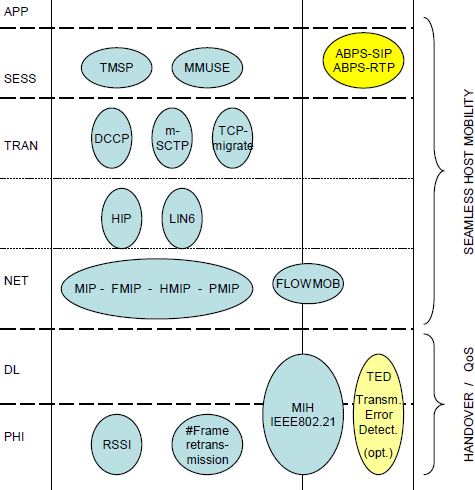
\includegraphics[width=10cm]{img/panoramica-soluzioni}
  \caption{\em Panoramica delle soluzioni e loro collocazione ai vari
    livelli dello stack ISO/OSI}
  \label{fig:panoramica}
\end{figure}

\section{Soluzioni \emph{single layer}}
Le architetture seguenti sono dette \emph{single layer} perché hanno
una collocazione ben precisa nello stack ISO/OSI e operano soltanto al
loro livello di appartenenza. L'analisi di queste soluzioni mostrerà i
limiti dell'approccio single layer, limiti che saranno superati dagli
approcci \emph{cross layer} descritti nella sezione successiva.

Queste architetture coprono i principali strati dello stack ISO/OSI:
Mobile IPv6 \cite{bib:mipv6} e la sua estensione Multiple Care-of
Addresses Registration \cite{bib:mcoa} agiscono a livello
\emph{network}, Host Identity Protocol \cite{bib:hip} definisce un
livello aggiuntivo tra \emph{network} e \emph{transport}, Datagram
Congestion Control Protocol \cite{bib:dccp} e Mobile Stream Control
Transport Protocol \cite{bib:m-sctp} lavorano a livello
\emph{transport}, infine Terminal Mobility Support Protocol
\cite{bib:tmsp} e MMUSE \cite{bib:mmuse} agiscono a livello
\emph{session}.

\subsection{Mobile IPv6 e Multiple Care-of Addresses Registration}
* Home Agent nella rete fa da LR\\
* Host parlano IPv6\\
* quindi infrastrutture di rete attuali non sono adatte\\
* no multi homing, perche' il protocollo non lo permette\\
* handover tribolato\\
MCoA\\
* estensione di MIPv6\\
* permette a MN di registrare più IP address con il suo Home Agent\\
* FlowMob permette di separare flussi di traffico tra le varie NIC\\
* stessi problemi di MIPv6: tutte le infrastrutture da cambiare.

\subsection{Host Identity Protocol}
* server tipo DNS opera fuori dalla rete di accesso\\
* mappa identificatori a posizioni\\
* il layer aggiuntivo deve essere installato sia nel MN che nel
  CN.\\
* Poco pratico! Non è detto che il CN si prenda la briga di installare\\
  il layer aggiuntivo.\\

\subsection{Datagram Congestion Control Protocol}
* ogni MN annuncia il cambiamento di rete all'altro nodo\\
* funziona solo se cambiano rete uno alla volta! Due MN che cambiano
  rete simultaneamente sono irragiungibili.\\
* richiedono modifica delle applicazioni.\\

\subsection{Mobile Stream Control Transport Protocol}
Idem a DCCP.

\subsection{Terminal Mobility Support Protocol}
* SIP user agent pubblico fuori dalle reti di accesso, mappa
  user@foo.com a posizione\\
* handover lento! ogni riconfigurazione interrompe la comunicazione
  finchè MN non ha finito di comunicare con l'user agent pubblico.

\subsection{MMUSE}
* server SIP, Session Border Controller (SBC) all'interno del
  sistema autonomo, che può essere composto da più reti wireless
  eterogenee.\\
* permette di attraversare i firewall e di spostarsi da una subnet
  all'altra all'interno dello stesso AS.\\
* MN non si può muovere tra reti di diversi AS.\\

\subsection{Considerazioni}
Tutte soluzioni tranne MMUSE hanno problemi con NAT e
firewall. Bisogna usare TURN e STUN. Tutte soluzioni senza
multi-homing, tranne MCoA.

\section{Soluzioni \emph{cross layer}}
Queste architetture sono dette \emph{cross layer} perché agiscono a
multipli livelli dello stack ISO/OSI, superando i limiti delle
architetture \emph{single layer} descritte in precedenza.

Il concetto di fondo di queste architetture è utilizzare le
informazioni disponibili al livello \emph{data link} per poter
prendere decisioni efficaci di qualità di servizio ai livelli più
alti, come trasporto o sessione.

Questa sezione confronterà le soluzioni ``Media Optimization Network
Architecture'' (MONA) e ``Always Best Packet Switching'' (ABPS).

Entrambe le architetture agiscono in uno scenario in cui ci sono
numerosi Mobile Node (MN), ognuno dotato di più interaccie di rete
(NIC), che operano in un ambiente dove sono disponibili più reti
wireless, eterogenee per tecnologia e dominio. Si immagina che i
movimenti degli utenti portino i vari MN ad attraversare le aree di
copertura delle reti wireless, per cui un MN connesso ad una
determinata rete A potrebbe spostarsi in un'area in cui giungono sia i
segnali della rete A che quelli di una seconda rete B, per poi
spostarsi ulteriormente nell'area di copertura della sola rete
B. Durante questi spostamenti l'utente deve essere in grado di
utilizzare applicazioni di rete real time, come Voice over IP e Video
on Demand, senza avere ripercussioni sulla qualità dell'esperienza. Il
traffico real time deve inoltre coesistere con il traffico non real
time delle applicazioni TCP/IP tradizionali, senza per questo venirne
penalizzato.

\subsection{Media Optimization Network Architecture}
%% Breve panoramica di MONA

MONA definisce uno strato aggiuntivo, posizionato tra gli strati
\emph{network} e \emph{transport} e denominato \emph{association
  layer}, che implementa l'Association Management Protocol (AMP);
detto protocollo risiete degli host e ne gestisce i singoli
collegamenti di rete, nascondendone la molteplicità allo strato
\emph{transport} superiore.

La molteplicità di collegamenti viene sfruttata per gestire il
problema dell'\emph{handover}, ovvero del passaggio dall'associazione
con una rete all'associazione con un'altra. In MONA ogni NIC tenta di
associarsi al proprio access point, e AMP decide se utilizzare una
sola NIC, quando il collegamento è soddisfacente, o se utilizzarne più
d'una contemporaneamente, quando il monitoraggio della NIC mostra
problemi di degrado delle prestazioni di rete.

MONA inoltre propone una modifica al comportamento degli access point
per supportare più efficientemente il traffico bidirezionale tipico
delle applicazioni VoIP e una aggiunta alle frame di \emph{probe} e
\emph{beacon} per permettere ai MN di selezionare l'access point con
migliore \emph{throughput}.


\subsection{Always Best Packet Switching}
%% Breve panoramica di ABPS

TODO

Fixed server, rappresenta MN. Uso simultaneo di tutte le
NIC. Scorciatoie SIP per evitare dialoghi lenti con server
SIP. Sicurezza e identificazione: pre-shared key, flow-id e niente
REINVITE. Meccanismi a disposizione per diverse politiche: VoIP usa
error detection ed early retransmission, VoD usa più NIC
contemporaneamente per maggior banda: virtual channels per selezionare
politiche. Estensioni: ABPS-SIP e ABPS-RTP.


\subsection{Considerazioni}
Vantaggi delle due soluzioni rispetto a quelle single layer.

\clearpage{\pagestyle{empty}\cleardoublepage}


\chapter{Media Optimization Network Architecture}

Media Optimization Network Architecture (MONA) è un progetto di un
gruppo di ricercatori giapponesi appartenenti all'Institurte of
Information and Communication Technology, Nara Institute of Science
and Technology, Kyushu Institute of Technology e Tokio Institute of
Technology.

In previsione dello sviluppo delle reti ubique, MONA affronta i
problemi descritti nella sezione \ref{sec:punti-critici} con un
approccio multihoming e cross layer.

La maggior parte del sistema MONA si concentra sul QoS dei
collegamenti \emph{first hop}, ovvero i link wireless.

I requisiti di MONA per avere una buona qualità di servizio sono:
1) iniziazione dell'handover basata sul rilevamento delle
caratteristiche del link wireless, 2) eliminazione dell'interruzione
dovuta all'handover, 3) selezione dell'interfaccia ottimale.

Sfruttando più interfacce di rete, MONA affronta il problema
dell'eterogeneità dei collegamenti, permettendo flussi di dati
multipli e fornendo QoS per ognuno; le NIC multiple permettono inoltre
di gestire l'handover in modo trasparente.

L'handover viene effettuato quando il collegamento wireless in uso
viene giudicato non più soddisfacente. Per determinare la qualità di
un collegamento, MONA misura il numero di ritrasmissioni a livello
data link.

Per gestire la molteplicità di NIC e i cambi di indirizzo IP dovuti
agli handover, MONA inserisce un nuovo layer chiamato
\emph{association layer} tra il livelli rete e trasporto. Il
protocollo relativo, denominato Association Layer Protocol (AMP),
aggrega e gestisce i flussi di dati tra gli endpoint inserendo
segnalazioni di modifica di stato e informazioni di identificazione.

Considerando che le applicazioni VoIP generano un traffico simmetrico
in uplink e in downlink e che il protocollo 802.11 è stato progettato
per ottimizzare il downlink, MONA propone una modifica al protocollo
per migliorare la bidirezionalità del traffico.

Per ultimo, per evitare che alcuni access point siano sovraccarichi di
collegamenti mentre altri rimangono inutilizzati, MONA propone un
algoritmo decentralizzato per distribuire i collegamenti tra gli
access point.

Le sezioni successive analizzeranno in dettagli questi punti.

\section{Association layer}

L'Association Layer (AL) di MONA è uno strato di associazione inserito
tra i livelli rete e trasporto AL è stato implementato in questa
posizione della pila dei protocolli per motivi di compatibilità. Come
mostrato dalla figura \ref{fig:mona-association-layer}, lo strato di
associazione è superiore allo strato di rete e non interferisce con lo
stack di protocolli di dispositivi come router e access point; in
questo modo MONA può funzionare senza modifiche agli apparati di rete.

\begin{figure}
\centering
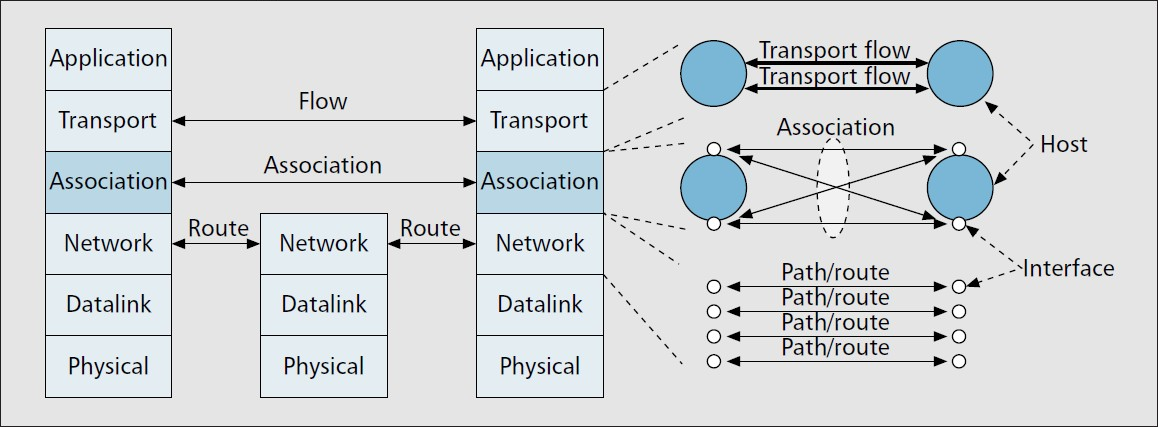
\includegraphics[width=\textwidth]{img/mona-association-layer}
\caption{\em Association layer di MONA}
\label{fig:mona-association-layer}
\end{figure}

Il protocollo Association Management Protocol (AMP) viene impiegato
dall'association layer per gestire gli stati delle associazioni tra i
vari host. Lo stato di ciascuna associazione può essere Inattivo
(Idle) quando non c'è comunicazione tra peer, Associato (Associated)
quando i due peer stabiliscono un'associazione attraverso il
three--way handshake di AMP, oppure Non Associato (No Association),
quando uno dei due peer non è in grado o rifiuta di stabilire
un'associazione. In quest'ultimo caso il layer di associazione
permette comunque la comunicazione tra gli host, assumendo un
comportamento trasparente; in altre parole, quando il tentativo di
associazione non va a buon fine, i peer comunicano attraverso lo stack
tradizionale, senza che l'estensione di associazione venga
utilizzata. Questo non permette di avere QoS tra i due peer, ma almeno
non impedisce le comunicazioni tra i dispositivi che implementano
l'Association Layer e i dispositivi tradizionali. Questa scelta
dovrebbe aiutare l'inserimento graduale dell'architettura nel mercato.

Quando due peer effettuano con successo un handshake AMP, lo strato di
associazione crea un'astrazione in cui tutti i flussi di rete tra i
due peer vengono raggruppati. Tale astrazione viene semplicemente
chiamata associazione e permette di ottimizzare le risorse di rete
condividendo le informazioni di identità dell'host tra i vari flussi
associati. L'associazione evita quindi all'host di dover ricorrere a
segnalazioni individuali per flusso ogniqualvolta venga eseguito un
handover: è infatti AL che, attraverso AMP, notifica le identità dei
flussi e delle interfacce di rete ai vari peer.

Nel caso in cui tra due peer venga stabilita un'associazione, il layer
inserisce in ogni pacchetto in uscita un header AMP posto tra l'header
e il payload IP, in modo da marcare ogni pacchetto dei flussi
dell'associazione. Tuttavia, secondo il protocollo AMP, i pacchetti di
controllo e di gestione, come le notifiche di instaurazione e di
terminazione dell'associazione, possono essere inviati
indipendentemente dai pacchetti di traffico, in modo che il layer di
associazione non debba attendere l'invio dei dati da parte degli
strati superiori per notificare il peer di eventi urgenti.

\section{QoS}
\label{sec:mona:qos}

La parte più interessante di MONA è la gestione della qualità del
servizio durante gli handover. MONA indica negli handover il punto
cruciale in cui si verifica la maggior percentuale di pacchetti persi
per un tempo abbastanza lungo da rendere impossibile la
comunicazione. Vengono considerati due tipi di packet loss: il primo
dovuto esplicitamente alla procedura di disattivazione e riattivazione
dell'interfaccia wireless durante il cambio di access point, come
descritto nella sezione \ref{sec:handover}, il secondo dovuto a
interferenze e collisioni tra pacchetti inviati da MN diversi.

Per evitare il periodo di inattività dovuto all'handover, MONA propone
di utilizzare più di un'interfaccia di rete sul MN, in modo che
durante il periodo di inattività di una, le altre siano in grado di
comunicare. Per esempio, mentre il MN sta comunicando con un peer
attraverso un'interfaccia di rete IF1, l'interfaccia di rete IF2
potrebbe cercare un'associazione di rete con un altro access point,
senza che questa attività influenzi la trasmissione dei dati
attraverso IF1. Se IF2 dovessere trovare un access point disponibile,
MN avrebbe due NIC collegate a Internet attraverso due reti
differenti; qualora il collegamento wireless di IF1 dovesse diventare
insoddisfacente, MN potrebbe dirottare il traffico in uscita da IF1 a
IF2, senza dover subire alcuna interruzione in quanto l'interfaccia
sarebbe già pronta all'uso.

MONA presenta un algoritmo per decidere quando è necessario passare
da l'invio di traffico su un'interfaccia all'invio di traffico su di
un'altra. Questo algoritmo misura la qualità del collegamento
attraverso il numero di ritrasmissioni a livello data link. Per
provare la validità di questo approccio, l'association layer di MONA e
il relativo protocollo AMP sono stati implementati nel simulatore di
rete Network Simulator 2 e sono stati condotti diversi esperimenti
virtuali per misurare l'efficacia dell'algoritmo e per determinare i
valori migliori di alcuni parametri.

Per prima cosa è necessario mostrare che il numero di ritrasmissioni a
livello data link sono una metrica per la misura della qualità di un
link più adatta dell'intensità del segnale radio.

\subsection{Ritrasmissioni L2 e intensità del segnale}

Secondo il protocollo 802.11 \cite{bib:802.11}, un nodo deve inviare
un ACK al peer ogniqualvota riceva un frame, in modo da confermare
l'avvenuta ricezione. Se il mittente non vede arrivare un ACK, ovvero
se il frame inviato o l'ACK stesso sono andati persi, allora
ritrasmette il frame. Questo meccanismo tenta la ritrasmissione del
frame fino a un numero prestabilito di volte: se il frame è più grande
di 2347 byte, viene ritrasmesso al massimo quattro volte, altrimenti
sette. Nel caso dell'architettura in questione il traffico in esame è
costituito da pacchetti VoIP, che sono di dimensione inferiore ai 400
byte; quindi ogni interfaccia ha a disposizione sette tentativi per
poter inviare il datagram VoIP all'access point. Se un link wireless è
in condizioni ottime, allora non si verificano mai errori di
trasmissione e i frame vengono inviati con successo al primo
tentativo. Quando le condizioni del link wireless cominciano a
peggiorare, possono cominciare a manifestarsi i primi packet loss, che
causeranno ritrasmissioni sporadiche. Infine, quando il link sarà in
condizioni critiche, le ritrasmissioni diverranno così frequenti da
raggiungere il limite di tentativi, provocando la perdita definitiva
del datagram.

Il primo esperimento simulato mira a trovare una relazione tra numero
di ritrasmissioni L2 e distanza del MN dall'AP. Se le due grandezze
sono correlate, allora le ritrasmissioni possono essere utilizzate al
posto della qualità del segnale. Il modello simulativo è costituito da
un MN che comunica con un CN via VoIP attraverso una rete 802.11b in
modalità infrastruttura. Entrambi i due host inviano pacchetti di 200
byte ad un intervallo di 20ms.

\begin{figure}
\centering
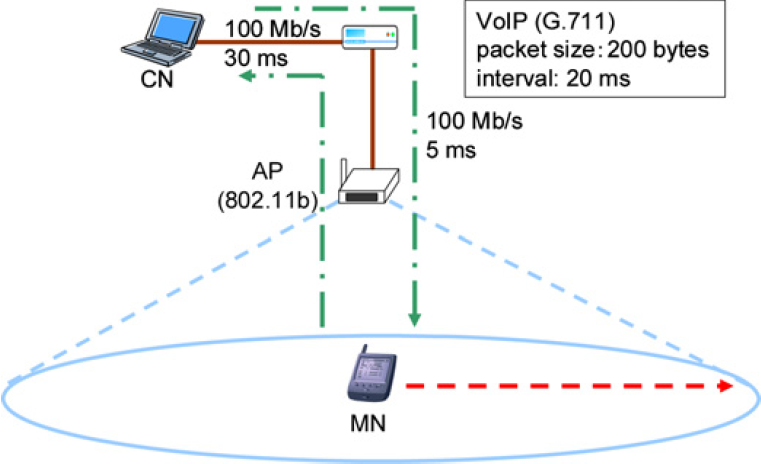
\includegraphics[width=\textwidth]{img/mona-distance-signal-strength-simulation}
\caption{\em Relazione tra distanza MN--AP e numero di ritrasmissioni e
  pacchetti persi: schema dello scenario e grafico dei risultati}
\label{fig:mona-distance-signal-strength-simulation}
\end{figure}

Il grafico della figura
\ref{fig:mona-distance-signal-strength-simulation} mostra come la
percentuale di pacchetti persi, ovvero di pacchetti scartati perché
hanno superato il numero massimo di ritrasmissioni, cresca rapidamente
a partire dalla distanza di 17 metri. Tuttavia si può notare che a
partire dai 15m le percentuali di pacchetti ritrasmessi aumentano fino
a poco sopra il 20\%. In questo scenario i 17m sono quindi la soglia
oltre la quale il segnale non è più abbastanza buono da garantire una
trasmissione senza packet loss; la simulazione mostra come il numero
di ritrasmissioni L2 permettono di rilevare questo problema prima di
incorrere nella perdita dei pacchetti. Come conclusione è lecito
affermare che il numero di ritrasmissioni L2 è una buona metrica su
cui basarsi per predirre il peggioramento del collegamento dovuto
all'indebolimento del segnale.

\subsection{Ritrasmissioni L2 e collisioni tra frame}

Poiché un secondo motivo per cui la qualità di un link wireless può
deteriorarsi è il verificarsi di collisioni tra frame spediti
simultaneamente da due o più MN, è stato condotto un esperimento per
indagare la relazione tra numero di ritrasmissioni L2 e collisioni tra
frame. Scopo della simulazione è mostrare che, eccedendo la banda
offerta da una rete wireless in modo da provocare collisioni, le
ritrasmissioni L2 aumentano di conseguenza.

Lo scenario descritto in figura \ref{fig:mona-collision-simulation} è
costituito da una rete 802.11b in cui vengono effettuate chiamate VoIP
con un numero progressivamente superiore di MN. Il traffico è
costituito da pacchetti di 200 byte inviati a intervalli di 20 ms. Dal
grafico si può notare che negli scenari in cui i MN sono presenti in
numero minore o uguale a dieci il numero di ritrasmissioni è prossimo
allo zero, mentre negli scenari in cui i MN sono undici o più il
numero di ritrasmissioni diventa via via sempre più considerevole.

\begin{figure}
\centering
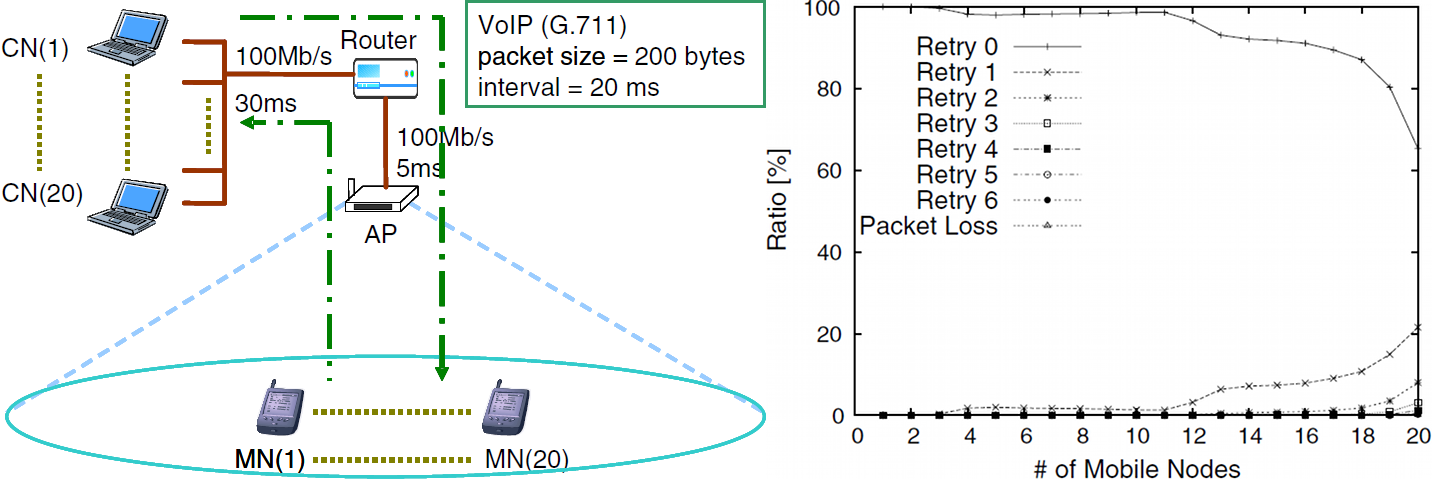
\includegraphics[width=\textwidth]{img/mona-collision-simulation}
\caption{\em Percentuale di pacchetti che vengono ritrasmessi in relazione
  al numero di MN: schema dello scenario e grafico dei risultati}
\label{fig:mona-collision-simulation}
\end{figure}

Considerando che una WLAN con banda 11MB/s può accomodare
approssimativamente 10 chiamate in cui pacchetti da 200 byte vengono
spediti a intervalli di 20ms \cite{bib:banda-wlan}, si vede che il
numero di ritrasmissioni aumenta proprio negli scenari in cui i MN
sono da undici a venti, ovvero le situazioni in cui la banda della
rete WiFI non è più in grado di reggere il carico di traffico. Questo
suggerisce che il numero di ritrasmissioni L2 è una buona metrica per
rilevare le condizioni in cui i link wireless sperimentano un alto
numero di collisioni perché la banda totale della rete wireless è
stata superata.

\section{Gestione dell'handover}

L'approccio cross--layer seguito da MONA consiste nel collezionare
informazioni sulla qualità dei link wireless a basso livello e fornire
questa informazione a uno strato superiore che decida quando e come
effettuare l'handover.

Come descritto nella sezione \ref{sec:mona:qos}, analizzare il numero
di ritrasmissioni di frame a livello data link può permettere di
predire il deterioramento di qualità di un link wireless. Questa
informazione è di basso livello, proveniendo appunto dal secondo
livello dello stack ISO/OSI. Decidere se effettuare l'handover, sulla
base di questa informazione, è invece una politica di alto livello,
che appartiene al componente aggiuntivo definito da MONA come Handover
Manager (HM). Questo componente viene implementato nello strato di
trasporto e utilizza le informazioni provenienti dal livello MAC.

\begin{figure}
  \centering
  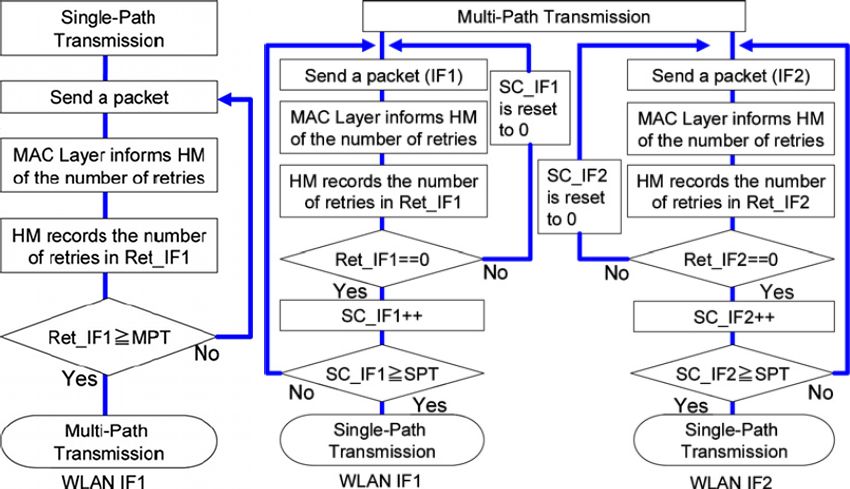
\includegraphics[width=\textwidth]{img/mona-sp-mp}
  \caption{\em Diagrammi di flusso che descrivono gli algoritmi usati da
    MONA per passare da Single Path Trasmission a Multi Path Trasmission
    (a sinistra) e viceversa (a destra).}
  \label{fig:mona:sp-mp}
\end{figure}

Nello schema proposto da MONA, quando un link viene rilevato come
problematico, l'Handover Manager utilizza le interfacce del MN
simultaneamente per prevenire il verificarsi di packet loss. Questo
utilizzo simultaneo viene chiamato Multi Path Trasmission (MPT) e
basilarmente offre sicurezza attraverso ridondanza. Quando uno dei
collegamenti in uso viene rilevato come stabile HM lo utilizza in modo
esclusivo, ritornando a quello che viene denominato Single Path
Transmission (SPT). Idealmente la modalità MPT dovrebbe essere attiva
per il tempo più breve possibile, perché l'utilizzo simultaneo di più
NIC può provocare un aumento di collisioni tra frame e determina un
aumento dei consumi di energia del dispositivo mobile.

\subsection{Da Single Path a Multi Path}

Come illustrato dal diagramma di flusso a sinistra nella figura
\ref{fig:mona:sp-mp}, si immagini un MN dotato di due interfacce
wireless IF1 e IF2. Allo stato iniziale MN comunica con il peer
attraverso l'uso esclusivo dell'interfaccia IF1; IF2 è attiva e
associata con un access point ma non riceve alcun datagram
dall'applicazione. Nel caso in cui IF2 non sia associata a nessun AP,
l'interfaccia scansiona alla ricerca di access point e si associa non
appena un AP diventa disponibile.

Durante l'uso di IF1, il MAC layer di IF1 informa HM del numero di
ritrasmissioni L2 che sono state necessarie per inviare ogni frame,
oppure comunica che il numero di ritrasmissioni massimo è stato
superato e che il frame è stato scartato. In questo modo HM viene a
conoscenza della condizione del link pacchetto per pacchetto ed è in
grado di decidere se la qualità del collegamento è diventata
insoddisfacente. Questa decisione viene presa confrontando il numero
di ritrasmissioni dell'ultimo frame, che nel diagramma è denominato
Ret\_IF1, con un valore soglia, superato il quale HM passa alla
modalità Multi Path Trasmission.

\subsection{Da Multi Path a Single Path}

Quando HM utilizza la modalità Multi Path Trasmission invia ogni
datagram ricevuto dall'applicazione a entrambe le interfacce,
raddioppiando il carico di rete e causando un incremento nelle
richieste energetiche del dispositivo mobile. Per questi motivi MPT
viene considerata una modalità d'emergenza, in cui HM deve operare per
il minor di tempo possibile.

Come in modalità SPT un alto numero di ritrasmissioni di un frame
viene considerato un indicatore del degrado di qualità del link, in
modalità MPT l'assenza di ritrasmissioni L2 viene considerato un
indice di stabilità del link. Il diagramma di destra della figura
\ref{fig:mona:sp-mp} mostra questo processo: ogni pacchetto viene
inviato simultaneamente su IF1 e IF2, che concorrentemente lo
inoltrano sul link wireless. Se il numero di ritrasmissioni di
un'interfaccia è zero, HM incrementa un valore denominato Stability
Counter (SC\_IFi), altrimenti lo reimposta a zero. Il valore SC viene
utilizzato come metrica discriminante per passare da MPT a SPT: quando
oltrepassa un certo valore soglia $s$ significa che il collegamento
wireless è stato in grado di inviare $s$ frame senza che fossero
necessarie ritrasmissioni, per cui può essere considerato stabile. La
prima interfaccia che giunge a una condizione in cui è considerata
stabile, viene selezionata da HM per essere utilizzata nuovamente in
modalità SPT.

Un problema introdotto dalla modalità MPT riguarda la ricezione di
paccheti duplicati dal peer del MN. Poiché lo stesso pacchetto viene
inviato su due interfacce connesse a reti differenti, i pacchetti
duplicati possono essere ricevuti fuori ordine, a causa delle diverse
condizioni delle due reti. La soluzione utilizzata in MONA marca ogni
pacchetto con un numero di sequenza, in modo che un nodo possa
scartare pacchetti ricevuti che possiedono un numero di sequenza
vecchio.

\section{Valutazione sperimentale}

Gli ideatori di MONA ne hanno valutato l'efficacia implementando
l'Handover Manager nel Network Simulator Version 2 \cite{bib:ns-2}
(versione 2.27) e conducendo una serie di simulazioni volte a
determinare se l'approccio funziona e quali valori soglia sono più
efficaci per gli algoritmi SPT/MPT.

\begin{table}
  \centering
  \begin{tabular}[bt]{|llll|}
    \hline
    Qualità & Buona & Media & Scarsa         \\
    \hline
    Delay (ms) & $<150$ & $150-400$ & $>400$ \\
    Jitter (ms) & $<20$ & $20-50$ & $>50$    \\
    Packet loss (\%) & $<1$ & $1-3$ & $>3$   \\
    \hline
  \end{tabular}
  \caption{\em Vincoli qualitativi considerati durante la simulazione.}
  \label{tab:mona:vincoli}
\end{table}

I vincoli qualitativi che sono stati considerati durante lo
svolgimento delle simulazioni per valutare la bontà dei risultati sono
riassunti in tabella \ref{tab:mona:vincoli}; l'obiettivo è di
mantenere la latenza tra i peer sotto i 150 ms, il jitter sotto i 20
ms e la percentuale di pacchetti persi sotto il l'1\%.

\subsection{Modello simulativo}

Gli esperimenti sono stati condotti sul modello schematizzato in
figura \ref{fig:mona:qos-sim-model}

\begin{figure}
  \centering
  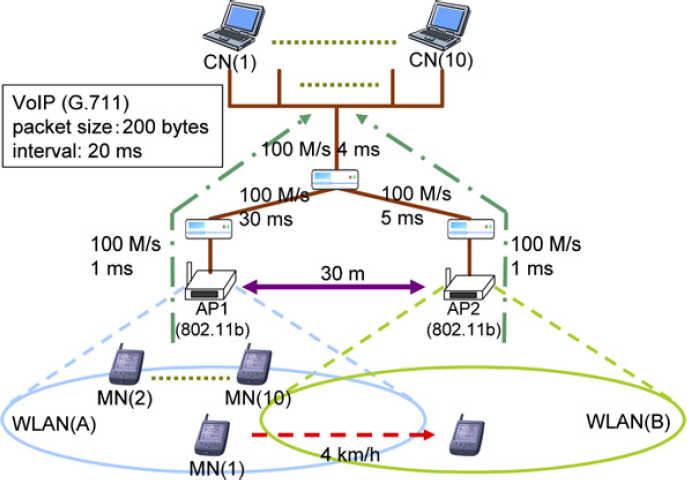
\includegraphics[width=\textwidth]{img/mona-qos-sim-model}
  \caption{\em Modello per la simulazione in NS2.}
  \label{fig:mona:qos-sim-model}
\end{figure}

Un Mobile Node (MN), equipaggiato con due interfacce di rete IF1 e
IF2, si sposta attraverso due WLAN differenti, ovvero dalla WLAN A
alla WLAN B. Durante l'handover vengono analizzati la percentuale di
pacchetti persi e il traffico di rete. Le due WLAN sono di tipo
802.11b e formano sottoreti differenti, in modo che le interfacce di
rete ricevano indirizzi IP diversi da ogni WLAN. Dieci MN sono
associati alla WLAN A e comunicano con altrettanti CN, mentre un solo
MN si sposta dalla WLAN A alla WLAN B, alla velocità di 4 Km/h, ovvero
a passo d'uomo. Tutti gli MN inviano pacchetti di 200 byte a
intervalli di 20 ms. Il delay tra peer è diverso a seconda della WLAN
a cui i MN sono associati: attraverso WLAN A è impostato a 35 ms,
mentre WLAN B 10 ms.

\subsection{Pacchetti persi}
\label{sec:mona:sim-packet-loss}

La prima analisi mira a individuare i valori migliori per le
ritrasmissioni di frame da utilizzare per le soglie di passaggio da
Single Path a Multi Path $v_{MPT}$ e da Multi Path a Single Path
$v_{SPT}$. Come da tabella \ref{tab:mona:vincoli} si sono cercati
valori in cui il packet loss misurato è minore del 3\%.

\begin{figure}
  \centering
  \begin{tabular}{cc}
    a) & 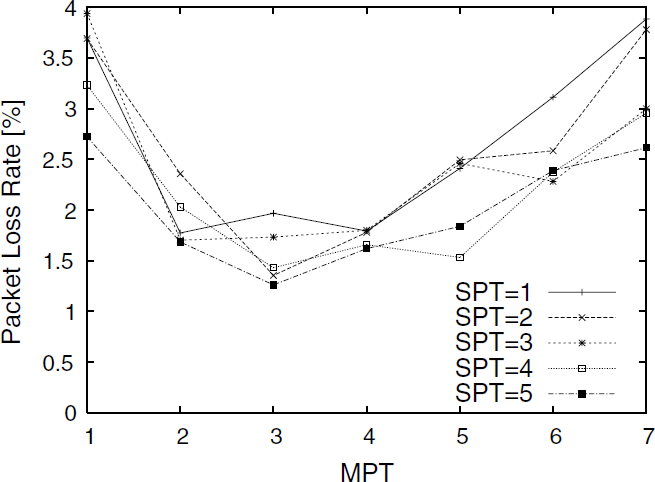
\includegraphics[width=9cm]{img/mona-sim-packet-loss-rate}  \\
    b) & 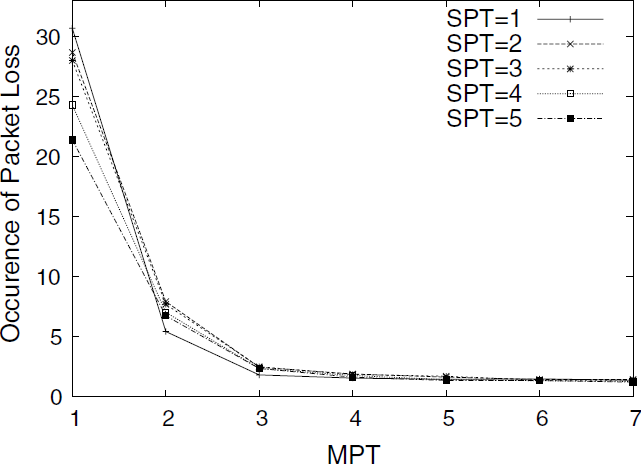
\includegraphics[width=9cm]{img/mona-sim-packet-loss-occur} \\
    c) & 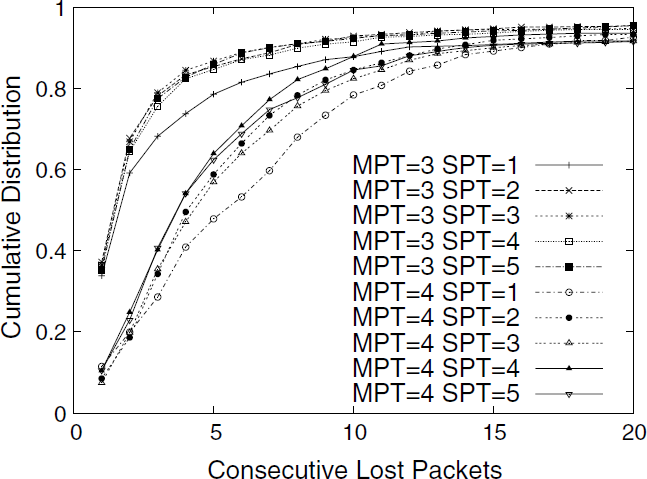
\includegraphics[width=9cm]{img/mona-sim-packet-loss-distrib}  \\
  \end{tabular}
  \caption{\em Misurazioni durante l'handover di a) percentuale di
    pacchetti persi, b) numero medio di occorrenze di pacchetti persi,
    c) distribuzione di pacchetti persi consecutivamente.}
  \label{fig:mona:qos-sim-packet-loss}
\end{figure}

Nel grafico a) della figura \ref{fig:mona:qos-sim-packet-loss} sono
mostrate le percentuali di pacchetti persi durante l'handover per
tutte le combinazioni di valori di SPT e MTP.  Le percentuali minori
del 2\% sono state misurate in corrispondenza dei valori 3 e 4 di MPT,
indifferentemente dal valore di SPT.  Che nella misura dei pacchetti
persi SPT sia un valore meno critico non stupisce, perché è il valore
che determina il ritorno alla modalità Single Path. MPT invece
determina il momento in cui HM passa alla modalità Multi Path e la
tempistica giusta è fondamentale. In particolare, si vede che quando
MPT è impostato a un valore troppo basso come 1 e 2, la percentuale di
pacchetti persi è alta come quando il valore è troppo alto (maggiore
di 4). Per approfondire il problema bisogna considerare il grafico b),
dove viene mostrato il numero di occorrenze di pacchetti persi, dove
ogni occorrenza è o un singolo pacchetto perso o una serie di
pacchetti persi. Dall'andamento del grafico si vede che con valori MPT
minori di 3 il numero di occorrenze è molto alto, ovvero ci sono
tanti pacchetti persi singolarmente, mentre per valori di MPT maggiori
di 4 il numero di occorrenze è molto basso; correlando questo dato con
quello del grafico a) dove la percentuale di pacchetti persi per
valori di MPT maggiori di 4 è molto alto, si conclude che con MPT alto
la comunicazione soffre di perdita di sequenze intere di pacchetti.

La spiegazione è da ricercarsi nella conformazione della rete: WLAN B
ha una latenza minore di WLAN A e i paccheti inviati attraverso di
essa arrivano prima dei pacchetti inviati attraverso la prima. Quando
HM è nel suo stato iniziale, invia numerosi pacchetti attraverso
l'interfaccia associata con WLAN A. L'access point relativo deve
gestire questo traffico insieme a quello degli altri dieci MN, per cui
i tempi di accodamento nel buffer del dispositivo cominceranno ad
essere rilevanti. Quando MPT ha un valore alto, HM attende che le
ritrasmissioni L2 arrivino al limite massimo e solo in quel momento
passa alla modalità Multi Path; passando a tale modalità invia un
frame attraverso WLAN B mentre nella coda di trasmissione dell'access
point sono ancora presenti numerosi frame precedenti. Poiché WLAN B ha
una latenza migliore e una congestione migliore di WLAN A, l'ultimo
frame arriverà a destinazione prima dei frame precedenti ancora
accodati; questi frame al loro arrivo verranno scartati come scaduti
perché hanno un numero di sequenza minore dell'ultimo pacchetto
ricevuto dal MN.

Nelle comunicazioni VoIP la perdita di una sequenza di pacchetti è più
grave della perdita di un pacchetto singolo. Analizzando la
distribuzione delle sequenze di pacchetti persi nel grafico c) della
figura \ref{fig:mona:qos-sim-packet-loss}, si nota che i valori più
bassi si hanno con MPT uguale a 3 e SPT uguale a 4.

\subsection{Carico di rete}

Se da una parte è necessario trovare i valori di MPT e SPT che
permettano di soddisfare al meglio i requisiti di QoS della tabella
\ref{tab:mona:vincoli}, dall'altra la modalità Multi Path è onerosa in
termini di carico di rete ed è necessario trovare un compromesso tra
qualità e utilizzo del medium.

\begin{figure}
  \centering
  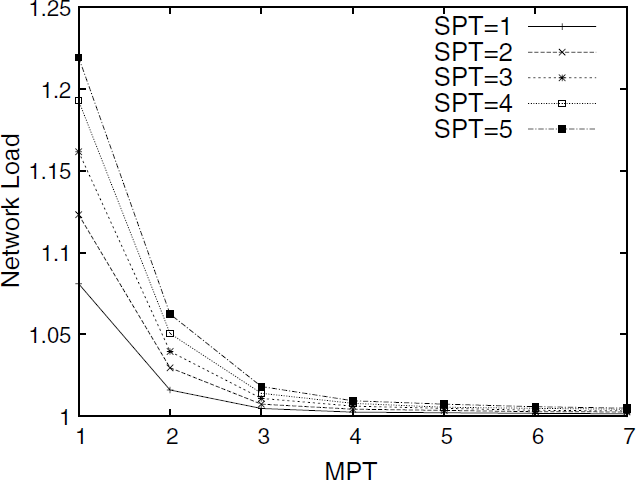
\includegraphics[width=10cm]{img/mona-sim-network-load}
  \caption{\em Analisi del traffico di rete durante l'handover}
  \label{fig:mona:sim-network-load}
\end{figure}

La figura \ref{fig:mona:sim-network-load} mostra i diversi carichi di
rete in relazione alle varie combinazione di MPT e SPT. Quando sia MPT
che SPT sono piccoli il carico di rete è relativamente basso, perché
HM passa facilmente alla modalità Multi Path, ma ritorna altrettanto
facilmente alla modalità Single Path. In contrasto, il carico di rete
massimo si ha quando MPT è basso e SPT è alto, perché HM passa
immediatamente in Multi Path e torna a Single Path con molta
difficoltà. Dalle prove condotte precedentemente (sezione
\ref{sec:mona:sim-packet-loss}) i valori più appropriati per MPT e SPT
sono risultati rispettivamente 3 e 2 e con queste costanti il carico
di rete durante il Multi Path è solo 1,004 volte il carico in Single
Path; in numeri, con un traffico di 80 kb/s in Single Path si ha un
traffico di 80,32 kb/s in Multi Path. Questo dimostra che i valori più
adatti a fornire QoS sono pienamente accettabili dal punto di vista
dell'incremento del carico di rete.

\subsection{Variazione nel ritardo dei pacchetti}

La variazione nel ritardo dei pacchetti, comunemente detta
\emph{jitter}, è un fenomeno che influenza la qualità delle
comunicazioni VoIP e dovrebbe essere al di sotto dei 50 ms, come da
tabella \ref{tab:mona:vincoli}. Nonostante MONA punti a mitigare la
perdita di pacchetti, è stato studiato l'effetto dei differenti valori
di MPT sul jitter.

\begin{table}
  \centering
  \begin{tabular}[bt]{|lllllll|}
    \hline
    Ritrasmissioni & 1 & 2 & 3 & 4 & 5 & 6                 \\
    \hline
    Jitter (ms) & 11,6 & 22,9 & 35,4 & 50,6 & 70,8 & 91    \\
    \hline
  \end{tabular}
  \caption{\em Jitter medio in relazione alle ritrasmissioni L2.}
  \label{tab:mona:jitter}
\end{table}

La tabella \ref{tab:mona:jitter} mostra i valori di jitter
relativamente al numero di ritrasmissioni di frame. Per avere valori
accettabili sotto i 50 ms è necessario che le ritrasmissioni siano al
massimo tre. Oltre questo valore i pacchetti cominciano ad accodarsi
nel buffer dell'interfaccia e subiscono variazioni nel ritardo. Il
valore migliore di MPT selezionato dalle prove precedenti è tre,
quindi l'utilizzo di MONA dovrebbe migliorare anche gli effetti sul
jitter.

\begin{figure}
  \centering
  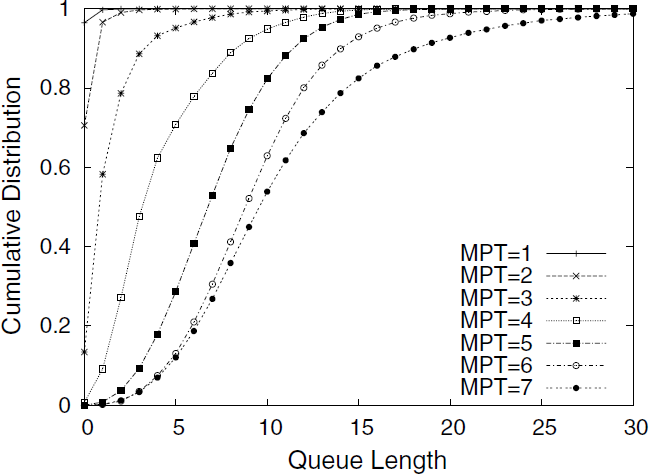
\includegraphics[width=10cm]{img/mona-sim-queue-length}
  \caption{\em Distribuzione cumulativa della lunghezza della coda di
    pacchetti nel buffer dell'interfaccia.}
  \label{fig:mona:sim-queue-length}
\end{figure}

La figura \ref{fig:mona:sim-queue-length} mostra la distribuzione di
probabilità della lunghezza della coda dei pacchetti nell'interfaccia
IF1 quando HM passa alla modalità MTP. Si può notare come a valori di
MTP crescenti la probabilità che la coda sia corta tenda a zero,
ulteriore conferma che i valori di MTP e jitter sono direttamente
correlati.

%% POSSIBILI AGGIUNTE

% Fair uplink and downlink in a WLAN.

% AP Selection: Load imbalance problem.

\section{Conclusioni}

TODO.

\clearpage{\pagestyle{empty}\cleardoublepage}

\chapter{Always Best Packet Switching}

Always Best Packet Switching è un progetto di ricerca dell'Università
di Bologna.

Gli obiettivi di ABPS sono: 1) identificare ogni MN in modo univoco in
ogni momento, a prescindere dalle reti a cui è connesso, 2) permettere
a un MN di essere raggiungibile da qualsiasi altro host e in
particolare da altri MN, 3) monitorare la qualità di servizio di ogni
canale di un MN per predire la necessità di un handover, 4) effettuare
detto handover in maniera trasparente, senza che la qualità del
servizio ne risenta. Perché la soluzione sia applicabile nella pratica
ABPS non richiede modifiche né agli apparecchi harware, né alle
applicazioni software esistenti.

L'architettura offre i servizi di QoS e sicurezza illustrati nella
sezione \ref{sec:punti-critici} alle applicazioni multimediali basate
sui protocolli SIP e RTP, con l'obiettivo di permetterne l'utilizzo in
un contesto di mobilità urbana attraverso reti eterogenee per
tecnologia, amministrazione e costo, anche con topologie di rete
contemplanti la presenza di NAT e firewall.

I vincoli di qualità del servizio che ABPS si impone di rispettare
sono gli stessi dichiarati da MONA nella tabella
\ref{tab:mona:vincoli} e indicati dalle raccomandazioni ITU-T G.1010
\cite{bib:itu-t}, ovvero massimo 150 ms di ritardo tra un estremo
della comunicazione all'altro e percentuale di pacchetti persi
inferiore al 3\%.

\section {Panoramica dell'architettura}
I problemi descritti nella sezione \ref{sec:punti-critici} vengono
affrontati da ABPS con un approccio cross--layer e distribuito. Cross
layer perché, come avviene in MONA, le informazioni raccolte al
livello MAC dei collegamenti wireless vengono messe a disposizione dei
livelli superiori perché possano prendere decisioni per la
salvaguardia della qualità del servizio; distribuito perché
l'architettura è composta da vari meccanismi software che cooperano in
diversi punti della rete per offrire i servizio di QoS, sicurezza e
mobilità. La figura \ref{fig:abps:arch} mostra una panoramica
dell'architettura.

\begin{figure}
  \centering
  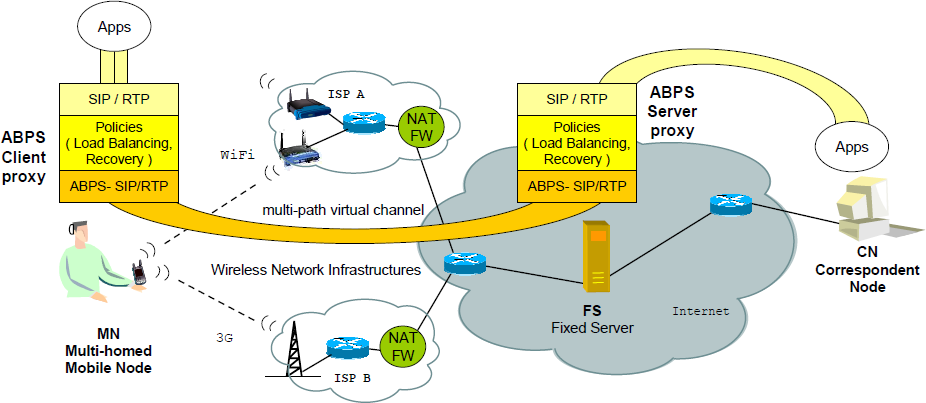
\includegraphics[width=\textwidth]{img/abps-arch}
  \caption{\em Architettura di ABPS}
  \label{fig:abps:arch}
\end{figure}

Nello scenario proposto da ABPS, il Mobile Node (MN) è dotato di più
d'una interfaccia di rete senza fili ed esegue applicazioni
multimediali basate sui protocolli SIP ed RTP. Le diverse reti senza
fili possono essere gestite da organizzazioni differenti e impiegare
apparati di rete che limitano la connettività, come firewall e
NAT. ABPS Server Proxy è un server pubblico raggiungibile direttamente
da Internet e indipendente dalle singole reti wireless e media ogni
comunicazione con il MN. Dall'altro estremo, il Correspondent Node
(CN) comunica con MN attraverso il proxy. Nella trattazione il CN è
raffigurato come un sistema tradizionale e non mobile per semplicità
d'esposizione, ma nulla vieta a un secondo MN di occupare il posto del
CN.

Il componente denominato ABPS Client Proxy viene eseguito sul sistema
del MN e si occupa di rispettare i vincoli di QoS monitorando i
collegamenti wireless e prendendo decisioni di recupero dagli
errori. Il componente denominato ABPS Server Proxy è invece un
servizio pubblico con cui ABPS--CP instaura un canale virtuale
costituito dai vari percorsi attraverso le reti wireless a cui le NIC
sono associate. Detto canale virtuale è un'astrazione fornita da
ABPS--SIP ed ABPS--RTP, estensioni rispettivamente dei protocolli SIP
ed RTP, ed è nascosto alla vista del CN dall'ABPS--SP; in questo modo
il CN non deve occuparsi della mobilità del MN ma può comunicare con
un rappresentante pubblico e dall'indirizzo IP fisso. Inoltre il
canale virtuale multipercorso offre servizi di identificazione dei MN
e di sicurezza dei flussi di traffico.

Caratteristica peculiare del funzionamento di ULB è che la scelta
dell'interfaccia più adatta viene effettuata pacchetto per
pacchetto. Questo è diverso da ciò che accade per esempio in MONA,
dove l'interfaccia viene selezionata solo quando offre garanzie di
qualità in maniera stabile e viene utilizzata in modo esclusivo fino a
che la qualità di servizio rimane accettabile; in ABPS un pacchetto
può essere inoltrato attraverso un'interfaccia, il pacchetto
successivo su un'altra e quello successivo su di un'altra ancora.

Dalla selezione dell'interfaccia effettuata pacchetto per pacchetto
nasce la possibilità di applicare politiche di instradamento
personalizzate per flusso. Per esempio, un flusso di traffico che
richieda una bassa latenza e poca banda potrebbe essere instradato su
un'interfaccia connessa a una rete con tariffa a volume di
traffico. Al traffico di una conversazione informale potrebbe invece
essere negato l'accesso ad ogni interfaccia connessa alle reti a
pagamento, permettendo l'instradamento esclusivamente sulle reti ad
accesso gratuito.

La possibilità di specificare politiche in termini di vincoli di
banda, latenza e costo economico è una caratteristica che ABPS
supporta mediante il concetto di canale virtuale. L'idea è che
ABPS--CP possa offrire numerosi socket all'applicazione SIP, ognuno
con una semantica di qualità di servizio diversa. In questo modo le
applicazioni possono essere collegate al socket che offre il servizio
desiderato. In altre parole, ad ogni socket viene associato un diverso
algoritmo di manutenzione della qualità di servizio, permettendo
all'applicazione e all'utente di decidere quale algoritmo debba essere
utilizzato semplicemente specificando il socket appropriato.

\begin{figure}
  \centering
  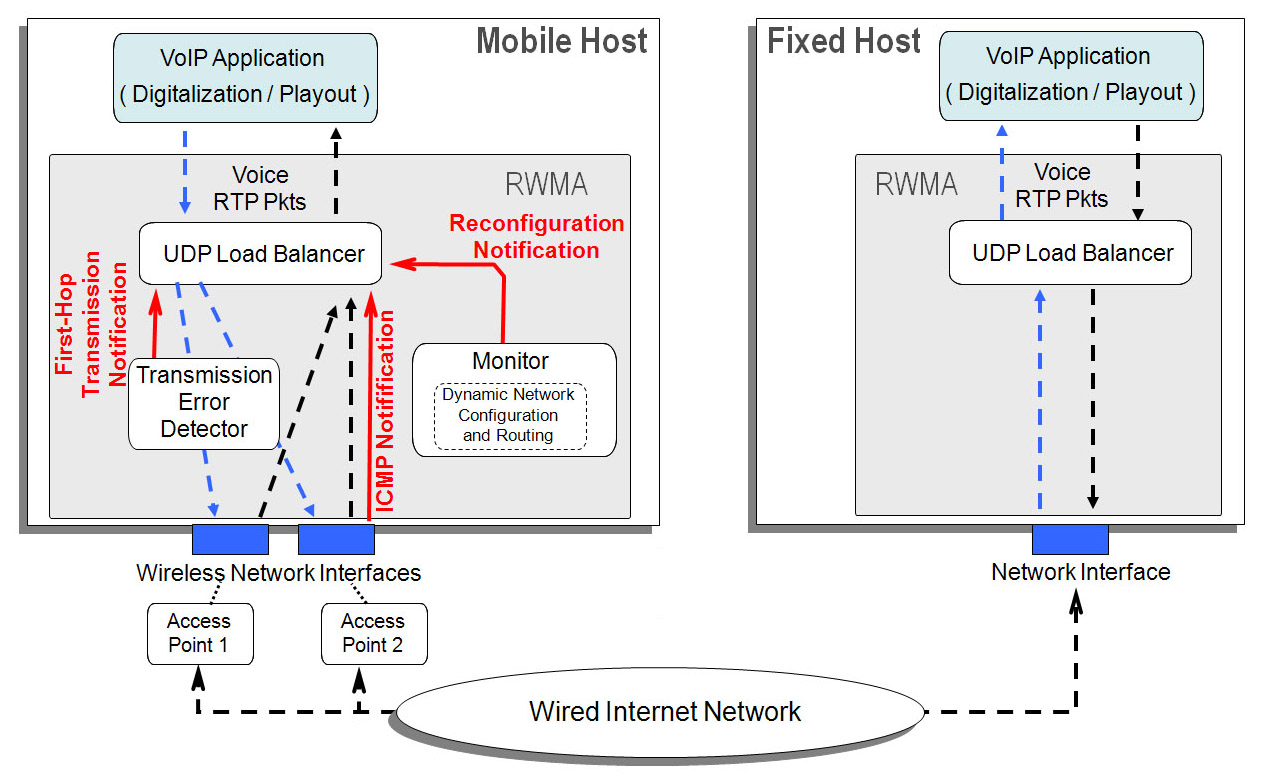
\includegraphics[width=\textwidth]{img/rwma}
  \caption{\em Meccanismi RWMPC del MN (a sinistra) e del CN (a
    destra).}
  \label{fig:abps:rwmpc}
\end{figure}

\section{Gestione della qualità del servizio}

Il cuore della gestione della qualità del servizio di ABPS è il
meccanismo Robust Wireless Multi--Path Channel (RWMPC), raffigurato
nella figura \ref{fig:abps:rwmpc}. RWMPC è essenzialmente uno strato
middleware che viene implementato negli host agli estremi di una
comunicazione VoIP. La versione sperimentale di RWMPC è stata
sviluppata nel kernel Linux 2.6.27.4, su una distribuzione Gentoo. I
componenti che costituiscono il meccanismo sono Trasmission Error
Detection (TED), UDP Load Balancer (ULB) e Monitor. TED si occupa di
rilevare gli errori a livello MAC nell'invio dei dati sull'interfaccia
di rete wireless, per poi notificare l'UDP Load Balancer. UDP Load
Balancer si occupa di ritrasmettere i datagram persi in base alle
notifiche di TED e decide qual è l'interfaccia wireless migliore da
utilizzare per l'invio dei dati. Monitor è il componente che configura
le interfacce del MN quando si attivano e si disattivano per
notificare ULB delle interfacce wireless disponibili. Le sezioni
successive analizzeranno il funzionamento dei componenti in dettaglio.

\begin{figure}
  \centering
  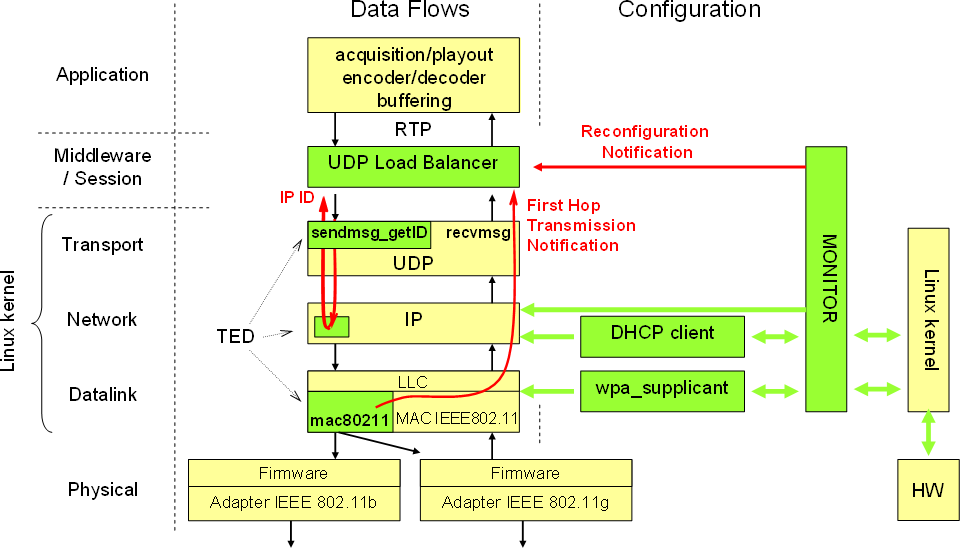
\includegraphics[width=\textwidth]{img/abps-rwmpc-funzionamento}
  \caption{\em Dettaglio dei componenti di RWMPC}
  \label{fig:abps:rwmpc-funzionamento}
\end{figure}

\subsection{Transmission Error Detector}

Il Transmission Error Detector (TED) è un componente che agisce nello
stack di protocollo del MN, operando nei livelli data link, rete e
transporto. Responsabilità principale di TED è monitorare l'invio di
ogni pacchetto e notificare UDP Load Balancer dell'esito di ogni
trasmissione. Per svolgere questo proprio compito TED si basa sul
meccanismo di ACK definito dal protocollo 802.11: ogni volta che
un'interfaccia wireless invia un frame, attende un frame di conferma
di avvenuta ricezione dall'access point. Se il frame inviato o quello
di conferma sono stati persi, l'interfaccia ha a disposizione dai
quattro ai sette tentativi per inviare nuovamente il frame e ricevere
conferma. Esauriti i tentativi, il frame è considerato perso e lo
strato MAC lo scarta silenziosamente. Con TED la ricezione dell'ACK e
la perdita del frame non sono più silenziosi ma vengono comunicati
agli strati superiori, che possono così essere informati delle
condizioni del collegamento wireless.

\subsection{UDP Load Balancer}

UDP Load Balancer è un'applicazione software eseguita dal sistema
operativo del MN che è responsabile dell'instradamento sulle diverse
interfacce di rete wireless dei pacchetti ricevuti dall'applicazione
SIP/RTP. Obiettivo di ULB è trasmettere i pacchetti applicazione
sull'interfaccia di rete che è giudicata essere la più adatta a
rispettare i vincoli di QoS. Le notifiche ricevute dal TED informano
dell'esito di ogni invio di pacchetto, perciò ULB è in grado di
decidere se ritrasmettere o meno un datagram che è stato scartato dal
livello MAC del MN. In base alle notifiche ricevute dal TED, ULB può
costruire una metrica su cui valutare la qualità del collegamento di
un'interfaccia di rete.

In aggiunta alle notifiche ricevute dallo strato data link, che
informano dello stato del collegamento nel primo segmento di rete, ULB
può ricevere le notifiche ICMP che informano sullo stato degli invii
dei datagram lungo tutto il percorso. Per esempio, dopo un handover il
MN si potrebbe ad inviare i dati attraverso una rete che per topologia
o politiche di accesso non permette al traffico di giungere fino al
CN. In questo caso, il link wireless potrebbe essere in condizioni
ottime, ma la rete non dovrebbe comunque essere utilizzata. Se i
messaggi ICMP non vengono bloccati, una notifica di tipo Destination
Unreachable permetterebbe a ULB di venire a conoscenza del problema,
mettendolo in condizione di agire in maniera correttiva (ad esempio
selezionando un'altra interfaccia per l'invio dei dati).

ULB riceve una terza tipologia di notifica dal componente Monitor,
descritto in seguito, che comunica a ULB qualsiasi cambiamento nello
stato delle interfacce di rete.

Mediante questi tre tipi di notifiche ULB viene a conoscenza dello
stato della situazione del MN e dei suoi collegamenti wireless e
prende decisioni di salvaguradia della QoS.

\subsection{Monitor}

Il componente Monitor è responsabile della configurazione delle
interfacce wireless del MN, notificando ogni cambiamento del loro
stato a ULB.

Normalmente le reti wireless forniscono un servizio DHCP che assegna
un indirizzo IP alle interfacce appena associate. Nei sistemi Linux
uno dei software disponibili per la gestione delle schede di rete
senza fili dei sistemi client è \emph{wpa\_supplicant}
\cite{bib:wpa_supplicant}; su di esso è basato Monitor, che sfrutta le
funzionalità esistenti e ne definisce di nuove. Monitor eredita la
gestione della sicurezza delle reti wireless, ad esempio WEP e WPA, la
scansione dei canali per la ricerca di un access point disponibile e
l'associazione con l'access point. Una modifica introdotta da Monitor
impedisce che due interfacce si associno allo stesso access point,
perché verrebbero a mancare tutti i vantaggi del
multihoming. Completata l'associazione con un access point, Monitor
utilizza un client DHCP per configurare l'indirizzo IP e
l'instradamento verso il gateway fornito. Quando la NIC è configurata,
Monitor invia una notifica di riconfigurazione (denominata
``Reconfiguration Notification'' in figura
\ref{fig:abps:rwmpc-funzionamento}) al processo ULB.

Quando l'interfaccia wireless perde il segnale con l'access point,
Monitor esegue il processo inverso: mediante wpa\_supplicant annulla
l'associazione con l'access point, rimuove le informazioni di routing
dell'interaccia dalla tabella di routing del MN e invia al processo
ULB una nuova notifica di riconfigurazione che specifica quale
interfaccia è stata disattivata in modo che ULB possa chiudere il
socket relativo.

\subsection{Selezione dell'interfaccia di invio}

L'algoritmo chiave per la gestione della qualità del servizio risiede
nel componente ULB, che ha la responsabilità di decidere per ogni
pacchetto ricevuto dall'applicazione quale sia l'interfaccia di rete
più adatta al suo invio.

La selezione dell'interfaccia di invio costituisce un problema
complicato perché richiede di valutare le varie interfacce secondo un
numero molto alto di parametri, sia lato rete che lato applicazione.

Lato rete ULB deve considerare le metriche di qualità del servizio di
affidabilità e interattività già viste; basandosi sulle notifiche del
componente TED, ULB può costruire una classifica di interfacce dalla
più affidabile alla meno affidabile.

Lato applicazione il problema è più complesso perché le richieste
possono diventare arbitrariamente complicate. Ad esempio
un'interfaccia di rete può avere un costo economico legato al volume
di traffico inviato o al tempo di utilizzo. In questo caso l'utente
potrebbe preferire che un'interfaccia di questo tipo venisse
utilizzata solo in caso di estrema necessità, anche se dovesse essere
l'interfaccia più affidabile; ULB si troverebbe quindi a dover
scegliere tra due vincoli contraddittori: lato rete l'affidabilità
dell'interfaccia la renderebbe ideale per l'invio dei pacchetti,
mentre lato utente il costo economico la renderebbe poco desiderabile
se non in particolari condizioni di estrema urgenza.

Attualmente l'algoritmo di selezione di ULB si basa esclusivamente
sulle metriche lato rete. ULB mantiene una lista di datagram da
inoltrare al CN, ordinati in base all'instante di tempo in cui sono
stati ricevuti dall'applicazione. Ogni interfaccia di rete ha un
socket UDP legato ad essa, in modo che ULB possa decidere l'utilizzo
di una NIC semplicemente selezionando il socket per l'invio del
datagram. Ogni socket ha uno stato associato, che descrive la
situazione della relativa interfaccia: \emph{working} significa che
l'interfaccia è funzionante ed affidabile ed è lo stato iniziale,
\emph{suspected} significa che l'interfaccia ha avuto un comportamento
problematico, infine \emph{disabled} se il componente Monitor informa
ULB che l'interfaccia non è più disponibile.

ULB seleziona un'interfaccia tra quelle in stato \emph{working} e
invia il datagram in cima alla lista attraverso il socket
associato. Le notifiche ricevute da TED informano ULB dello stato
dell'invio e possono scatenare un cambiamento di stato: se
un'interfaccia \emph{working} riceve una notifica di errore a livello
MAC, lo stato del socket associato diventa \emph{suspected}. Se invece
la notifica è di tipo ICMP o una riconfigurazione ricevuta da Monitor,
l'interfaccia diventa \emph{disabled}. Un'interfaccia in stato
\emph{suspected} non viene scelta per l'invio dei dati finché è
presente almeno un'altra interfaccia \emph{working}; in caso contrario
può essere scelta e se l'invio va a buon fine oppure se riceve un
datagram dal CN, ULB marca il socket associato come nuovamente
\emph{working}.

Per supplire alle mancanze di alcuni firmware di schede wireless che
non sono in grado di notificare che un frame è stato scartato dal MAC
layer, ULB mantiene un timeout di 30 ms ad ogni invio di frame. Se
entro questi 30 ms ULB non riceve notifiche da TED riguardo il
datagram appena inviato, ULB assume che il frame sia stato scartato e
marca il socket utilizzato come \emph{suspected}.

Il supporto per le politiche lato applicazione è in fase di studio e
prevede che ULB metta a disposizione delle applicazioni più coppie di
porte SIP/RTP, associando ad ogni coppia un algoritmo diverso di
selezione dell'interfaccia di invio. Ad esempio una coppia di porte
potrebbe essere utilizzata dalle applicazioni VoIP, che richiedono
alta interattività, bassa latenza e scarsa disponibilità di banda e
tutti i dati inviati attraverso quelle porte verrebbero trattati da un
algoritmo adatto a questi requisiti; un'altra coppia di porte potrebbe
invece essere utilizzata dalle applicazioni Video--on--Demand (VoD)
che al contrario necessitano di un buon quantitativo di banda e di un
differente algoritmo di QoS che si occupi di bilanciare il carico di
rete piuttosto che di rilevare gli errori. Utilizzando questa
soluzione si potrebbero implementare politiche lato utente e
applicazione senza richiedere modifiche ai software esistenti.

\section{Supporto per la mobilità}

La mobilità di un MN e la conseguente capacità di cambiare rete
wireless di appartenenza in maniera continuativa pongono i problemi di
identificazione e raggiungibilità esposti nella sezione
\ref{sec:punti-critici}. Come soluzione ABPS definisce delle
estensioni per i protocolli SIP ed RTP per mezzo delle quali creare un
canale virtuale multipercorso che collega il MN a un server proxy
pubblico, denominato ABPS Server Proxy. Il canale è detto virtuale e
multipercorso perché è in realtà un insieme logico di percorsi di rete
che hanno hanno origine ognuno da una diversa interfaccia di rete del
MN. Ogni percorso attraversa inizialmente la rete wireless a cui è
associata l'interfaccia di rete, per poi raggiungere ABPS Server Proxy
seguendo la topologia della rete. Il canale virtuale permette di
identificare i flussi di traffico del MN indipendentemente dalla rete
di associazione, e quindi dall'indirizzo IP, della scheda di rete in
uso, in modo che il procedimento di handover non renda irragiungibile
il dispositivo mobile. I meccanismi del canale virtuale sono stati
progettati per funzionare entro i limiti di tempo richiesti dai
vincoli qualitativi, evitando quindi meccanismi intrinsecamente lenti
come handshake e interrogazioni client/server.

\subsection{Limiti del protocollo SIP}

Il protocollo SIP è utilizzato per creare il contesto di una
comunicazione tra due o più entità di rete. Per mezzo di SIP due host
possono venire a conoscenza l'uno dell'altro (ovvero conoscere i
rispettivi indirizzi IP) e accordarsi sui parametri della sessione di
comunicazione, dopo di che il trasferimento dati avviene in modo
diretto, secondo le modalità concordate. In questo approccio esistono
due problemi: 1) l'instaurazione della sessione è un meccanismo che
richiede un quantitativo di tempo che può essere accettabile
all'inizio della conversazione VoIP ma che risulta deleterio quando
deve essere effettuato dopo un handover, in corso di conversazione; 2)
la necessità che i sistemi in comunicazione siano mutuamente
raggiungibili in modo diretto rende impossibile il trsferimento dati
in reti che impiegano tecnologie di controllo del traffico come
firewall e NAT.

ABPS estende il protocollo SIP, utilizzato per l'istaurazione e il
mantenimento della sessione, e il protocollo RTP, utilizzato per lo
scambio di dati tra gli host, aggiungendo caratteristiche che mirano a
superare detti limiti.

Tra i vari ruoli che SIP prevede per gli host in gioco, la trattazione
di ABPS richiede di illustrare gli User Agent Client (UAC), gli User
Agent Server (UAS) e i Back-to-back User Agent (B2BUA).

\paragraph{User Agent Client.}
È definito come un'entità logica che crea nuove richieste SIP e le
invia attraverso la rete all'User Agent Server. Per esempio,
un'applicazione VoIP che inizi una chiamata prende il ruolo di UAC,
perché genera e spedisce la richiesta di invito.

\paragraph{User Agent Server.}
È definito come un'entità logica che crea le risposte alla richieste
ricevute. Un esempio di UAS è il server che risponde alle richieste di
registrazione degli utenti (Registrar).

\paragraph{Back-to-back User Agent.}
È definito come un'entità logica che riceve le richieste da un client
(UAC) e si comporta come se fosse un server (UAS), ma invece di
rispondere direttamente, inoltra la richiesta a un server (UAS); nel
dialogo con il client si comporta come server, mentre nel dialogo con
il server si comporta da client. In altre parole, un B2BUA è un
intermediario tra UAC e UAS: UAC crede che il B2BUA sia l'UAS,
dall'altra parte l'UAS crede che il B2BUA sia l'UAC.

In uno scenario VoIP, l'applicazione nel ruolo di UAC utilizza il
protocollo SIP per inviare al server (UAS) un messaggio REGISTER, per
segnalare che l'utente è collegato e pronto a ricevere e inviare
chiamate. Dopo che l'UAC si è registrato al servizio, può instaurare
una sessione mediante un messaggio INVITE, che specifica
l'identificativo dell'utente da contattare e i dati dell'utente
chiamante; ricevuta la richiesta INVITE, il server recupera
l'indirizzo IP dell'utente specificato e instaura una sessione tra i
due partecipanti, che possono comunicare direttamente mediante
protocollo RTP.

Nel caso in cui il chiamante modifichi il proprio stato durante una
conversazione, l'applicazione invia un nuovo messaggio INVITE
contentente i parametri aggiornati, per permettere al server di
reinstaurare la sessione con le nuove caratteristiche.

Il meccanismo di re-INVITE è intrinsecamente lento: il mittente deve
contattare il server, il server deve a sua volta contattare il
destinatario e solo a quel punto la comunicazione tra mittente e
destinatario può continuare nella nuova sessione. Nonostante questo
procedimento possa avvenire in automatico, ovvero senza intervento
manuale dell'utente, la comunicazione vocale deve essere interrotta
finché non viene instaurata la nuova sessione, condizionando
l'esperienza utente.

ABPS definisce delle scorciatoie di segnalazione per rendere diretto
il procedimento di re-INVITE; i partecipanti possono modificare i
parametri della sessione in cui sono coinvolti senza dover
interpellare il server e quindi evitando di dover attendere che la
sessione sia reinstaurata, evitando di inserire nel procedimento i
ritardi indesiderati che comprometterebbero la qualità della chiamata.

\subsubsection{Problematiche dovute a Firewall e NAT}

Il protocollo SIP si limita a creare il contesto della comunicazione,
permettendo ai partecipanti di conoscere i rispettivi indirizzi IP e
di concordare le caratteristiche della comunicazione. Poiché il
traffico di dati avviene in maniera diretta tra i due host, meccanismi
come NAT e firewall sono impedimenti alla comunicazione perché non
permettono a un host di essere direttamente raggiungibile dalla
controparte.

Nel contesto delle reti ubique, firewall e NAT sono verosimilmente di
proprietà dell'organizzazione che offre la connettività, per cui
l'utente non ha possibilità di ricorrere alle soluzioni di
port-forwarding che sono disponibili in contesti Small Office/Home
Office.

Un client che non sia in grado di essere direttamente raggiungibile su
Internet può utilizzare servizi come Traversal Using Relay NAT (TURN)
e Session Traversal Utilities for NAT (STUN).

STUN prevede che un server esterno, pubblicamente raggiungibile su
Internet, tenti diversi metodi per attraversare il NAT dietro al quale
si trova l'host che richiede connettività e, nel caso un metodo si
riveli efficace, la comunicazione può avvenire direttamente tra i due
host. L'algoritmo non è sempre efficace, in particolare non è in grado
di attraversare firewall simmetrici, e soprattutto richiede un certo
tempo per essere eseguito. Nel contesto delle reti ubique questo
metodo dovrebbe essere eseguito ad ogni handover, che nel caso di ABPS
avviene pacchetto per pacchetto; come conseguenza STUN non è una
soluzione accettabile perché il ritardo di cui necessita violerebbe i
vincoli di QoS.

TURN prevede un server esterno che si comporta come un relay, facendo
da intermediario per l'host schermato dal NAT per tutto il traffico
della comunicazione. Nello scenario in esame l'host è un dispositivo
mobile che cambia indirizzo IP in modo imprevedibile e TURN non ha
supporto per questo tipo di esigenza.

Per aggirare questi problemi di raggiungibilità tra gli host, ABPS
impiega quindi ABPS Server Proxy, essenzialmente un B2BUA SIP
modificato per supportare le estensioni SIP--ABPS e RTP--ABPS,
raggiungibile pubblicamente su Internet, che nasconde l'indirizzo IP
del MN e funge da intermediario pubblico per tutto il traffico del
MN. Grazie a questo B2BUA, i MN possono essere rappresentati da un
host pubblicamente raggiungibile su Internet, quindi evitando in
maniera semplice e sicura i problemi di NAT e firewall.

\section{Dettagli implementativi}

\subsection{ABPS Client Proxy}

ULB manda datagram, serve notifica esito.

TED usa 1) sendmsg\_getID che ritorna l'ID del datagram appena
spedito; 2) sistema di notifiche che riceve esito dal firmware e lo
comunica al socket applicazione attraverso error queue (abilitata con
IP\_RECVERR).

\subsection{ABPS Server Proxy}

\subsubsection{ABPS--SIP}

\subsubsection{ABPS--RTP}

\section{Valutazione sperimentale}

Un prototipo del meccanismo RWMPC è stato valutato con un esperimento
volto a determinare l'effettiva validità dell'algoritmo di
mantenimento del QoS. In particolare le prove miravano a misurare le
capacità di reazione di RWMPC ai cambiamenti di stato dei collegamenti
wireless, controllando che i vincoli di QoS, ovvero massimo 150ms di
ritardo nella consegna dei pacchetti e massimo 3\% di pacchetti persi,
non venissero infranti.

\begin{figure}
  \centering
  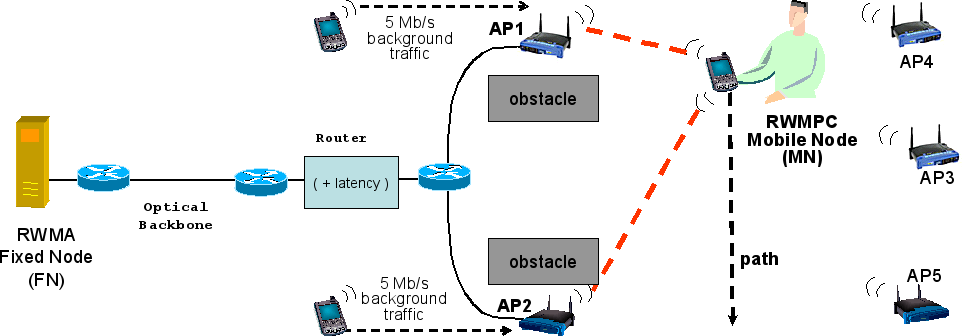
\includegraphics[width=\textwidth]{img/abps-simulazione}
  \caption{\em Scenario della simulazione sperimentale di RWMPC}
  \label{fig:abps:simulazione}
\end{figure}

L'esperimento si è svolto in uno scenario reale, raffigurato in figura
\ref{fig:abps:simulazione}. Un MN esegue il prototipo di RWMPC e si
muove in un ambiente in cui sono presenti quattro access point (in
figura AP1, AP2, AP3, AP4 e AP5). Di questi access point, solo AP1 e
AP2 forniscono connettività per MN, gli altri sono presenti solo per
generare interferenza di segnale. Gli ostacoli vicino agli access
point 1 e 2 sono posizionati in modo da schermare i segnali in modo
che non siano sovrapposti: all'inizio del percorso MN è in grado di
ricevere il segnale di AP1 ma non quello di AP2, mentre alla fine del
percorso avviene l'opposto. I due access point attivi ricevono
traffico di 5Mb/s da altri due MN, in modo da simulare la presenza di
altri dispositivi mobili. Il router a cui gli access point sono
connessi è stato impostato in modo da instradare i pacchetti che
riceve dopo una latenza casuale tra i 70 e gli 80 ms. Alla fine del
percorso c'è il CN fisso, che esegue una copia del prototipo RWMPC.

Il MN si sposta dalla copertura di rete di AP1 verso quella di AP2
inviando a intervalli di 40 ms dei frame di dimensione 160 B. Allo
stesso tempo, il CN invia pacchetti verso il MN con gli stessi
parametri di dimensione e tempo; il traffico simulato mira a ricreare
il carico di rete tipico di una conversazione VoIP bidirezionale a
32Kbps senza soppressione del silenzio. Durante lo spostamento del MN
la forza del segnale di AP1 e AP2 si inverte come da figura
\ref{fig:abps:delay-mn}. Come si può vedere, vicino ai 50 metri la
forza di segnale dei due AP si inverte, segnando il punto più critico
del percorso del MN.

\begin{figure}
  \centering
  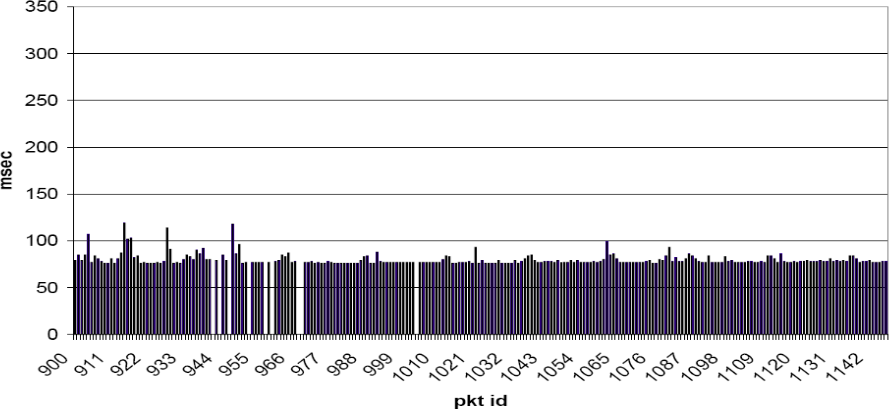
\includegraphics[width=\textwidth]{img/abps-delay-mn}
  \caption{\em Grafico del ritardo di ogni pacchetto ricevuto dal MN}
  \label{fig:abps:delay-mn}
\end{figure}

Le misurazioni effettuate sono mostrate nei grafici delle figure
\ref{fig:abps:delay-mn} e \ref{fig:abps-delay-cn}. In questi grafici,
ogni barra è il tempo impiegato dal pacchetto e una barra mancante
significa che il pacchetto non è stato ricevuto dall'host
corrispondente, perché si è perso durante il percorso e il meccanismo
RWMPC del CN non ritrasmette i pacchetti persi. Il grafico di figura
\ref{fig:abps:delay-mn} mostra il tempo che ogni pacchetto inviato dal
CN ha impiegato per giungere fino al MN; si può vedere che tutti i
pacchetti sono arrivati entro i 150 ms di limite e che solo una decina
di pacchetti, contro un totale superiore a mille, non sono giunti a
destinazione. Il grafico di figura \ref{fig:abps:delay-cn} mostra
invece il ritardo con cui il CN ha ricevuto i pacchetti inviati dal
MN; il meccanismo RWMPC del MN utilizza TED per rilevare gli errori di
invio delle interfacce wireless e rispedisce i pacchetti che sono
stati scartati dallo strato MAC, quindi tutti i datagram arrivano al
CN. Di questi, solo tre giungono oltre il limite massimo di 150 ms, e
sono da considerarsi persi perché in violazione dei limiti di QoS.

\begin{figure}
  \centering
  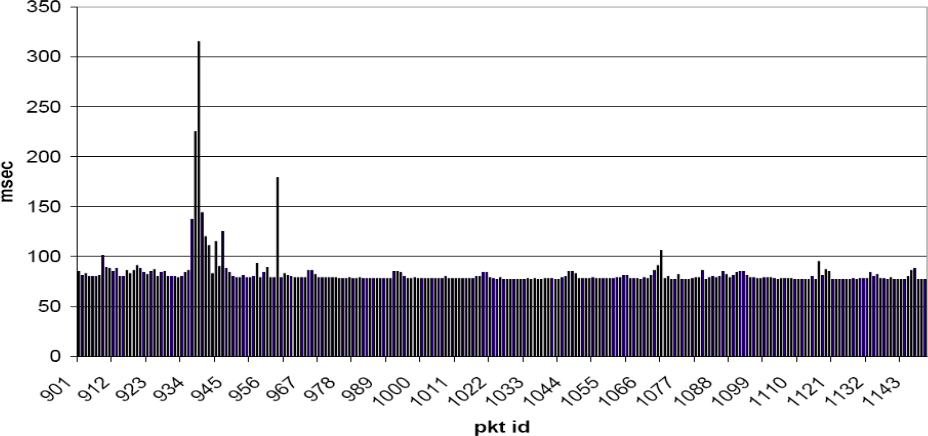
\includegraphics[width=\textwidth]{img/abps-delay-cn}
  \caption{\em Grafico del ritardo di ogni pacchetto ricevuto dal CN}
  \label{fig:abps:delay-cn}
\end{figure}

\section{Conclusioni}

TODO

\clearpage{\pagestyle{empty}\cleardoublepage}


\chapter{Considerazioni finali}
Riprende superiorità di cross layer su single layer e confronta punti
forti e deboli di MONA e ABPS.

Propone scenari di test?

\clearpage{\pagestyle{empty}\cleardoublepage}



\begin{thebibliography}{90}
\rhead[\fancyplain{}{\bfseries \leftmark}]{\fancyplain{}{\bfseries
\thepage}}
\addcontentsline{toc}{chapter}{Bibliografia}
\bibitem{bib:mipv6} RFC3775, ``Mobility Support in IPv6'',\\
  http://tools.ietf.org/html/rfc3775, giugno 2004
\bibitem{bib:misura-handoff-l2} A. Mishra, M. Shin, W. Arbaugh, An
  Empirical Analysis of the IEEE 802.11 MAC Layer Handoff Process, ACM
  SIGCOMM Computer Communication Review 33 (2), 2003.
\bibitem{bib:misura-handoff-dhcp} A. Dutta, F. Vakil, J. Chen,
  M. Tauil, S. Baba, N. Nakajima, H.  Schulzrinne, Application Layer
  Mobility Management Scheme for Wireless Internet, Proc. of IEEE 3G
  Wireless 2001, maggio 2001.
\bibitem{bib:mcoa} RFC5648, ``Multiple Care-of Addresses
  Registration'',\\http://tools.ietf.org/html/rfc5648, ottobre 2009
\bibitem{bib:hip} RFC5201 ``Host Identity Protocol'',\\
  http://tools.ietf.org/html/rfc5201, aprile 2008
\bibitem{bib:itu-t} ITU-T Recommendation G.1010, “End-user multimedia
  QoS categories,” November 2001
\bibitem{bib:banda-wlan} K. Medepalli, P. Gopalakrishnan, D. Famolari,
  and T. Kodama, Voice Capacity of IEEE 802.11b, 802.11a and 802.11g
  Wireless LANs, Proc. of Globecom 2004, pp.1549–1553, December 2004.
\bibitem{bib:abps} V. Ghini, G. Lodi, F. Panzieri, ``Always Best
  Packet Switching: the Mobile VoIP Case Study'', Achademy Publisher,
  Journal of Communications, accepted for publication.
\bibitem{bib:abc} E. Gustafsson et al., ``Always Best Connected'',
  IEEE Comm. Mag., vol. 10, no. 1, Feb 2003, pp. 49--55.
\bibitem{bib:ns-2} VINT Network Simulator 2,
  http://nsnam.isi.edu/nsnam/, ottobre 2009
\bibitem{bib:wpa_supplicant} Linux WPA Supplicant (IEEE 802.1X, WPA,
  WPA2, RSN, IEEE 802.11i), http://hostap.epitest.fi/wpa\_supplicant/,
  novembre 2009.
\end{thebibliography}

\clearpage{\pagestyle{empty}\cleardoublepage}

\chapter*{Ringraziamenti}
\thispagestyle{empty}
Grazie a Chiara per l'amore e la pazienza, ma soprattutto per l'amore
e la pazienza.

Grazie a Manuela, Claudio, Chiara, Tatiana e Michela.

Grazie alla mia famiglia che mi ha mantenuto e pagato gli studi.

Grazie al Dott. Vittorio Ghini per la disponibilità e la gentilezza.
\end{document}
